% Appendix: details for reproduction. Section labels are referenced from main.tex.

\section{Setup details}\label{app:setup}

\textbf{Scene.} The G1 model with Dex3 hands is taken from MuJoCo Menagerie~\cite{menagerie2022} at commit \texttt{c96a32d}. The pelvis is fixed to the world, gravity compensation is applied to the whole body (compensating only the right arm let the waist sag by about 4$^\circ$, which tilted the head camera), and the left arm is moved off the table. The head camera follows the D435i mount of the Unitree URDF (pitched about 48$^\circ$ down, vertical field of view 58$^\circ$). The part is one rigid body of two boxes (density 600\,kg/m$^3$, torsional friction enabled with \texttt{condim}=4); the flange box overlaps the body by 1\,mm.

\textbf{Visibility.} For a visible length $v$, the board front is placed so that the ray from the head camera through the lower front edge of the board meets the flange top surface $v$ behind the part's front face.

\textbf{Grasp motion.} The wrist is rolled $-60^\circ$, pitched $10^\circ$, and yawed $-55^\circ$ about the vertical, so that the pinch axis is almost lateral; the index finger is curled. Without a previous touch, the hand is inserted horizontally from 10\,cm in front of the board at 20\,mm above the grasp point, then lowered. After a touch, the hand moves under the board at or above its current height to above the grasp point. The thumb and middle finger close independently, each stopping at contact; once both touch, both close a further fixed amount over 0.3\,s. The hand then raises the part by 1\,cm, pulls it out to 10\,cm in front of the board, lifts it to 6\,cm above the grasp height, and holds for 2\,s. Moves near and under the board are straight lines in Cartesian space split into waypoints (15 by default; one per 1\,mm step during the touch descent and 12 for the withdrawal), each solved by mink~\cite{zakka2024mink}, with joint targets interpolated linearly in time. Moves in free space (the approach in front of the board and wrist re-orientation) solve inverse kinematics once and interpolate in joint space.

\textbf{Physics randomization.} Per layout: friction coefficient $\mu\sim U[0.3,1.0]$ on the fingers and the part (MuJoCo uses the larger of two contacting geoms), part mass and inertia scaled by $U[0.7,1.3]$, and the position gains of the hand actuators scaled by $U[0.8,1.2]$. MuJoCo's derived constants are recomputed after changing the mass; otherwise the simulation becomes unstable and success drops spuriously.

\textbf{Camera model.} Segmentation is the simulator's ground truth, corrupted by eroding or dilating the mask by one pixel (probability 1/3 each, otherwise unchanged) and flipping 30\% of the boundary pixels. Depth noise follows the D435i model $\sigma(z)=z^2\cdot0.08/(f b)$ with baseline $b=50$\,mm.

\textbf{Particle filter.} 3,000 prior candidates: front-face position $\mathcal{N}(\text{prior},\,(30\,\text{mm})^2)$ in depth and $\mathcal{N}(\text{prior},\,(15\,\text{mm})^2)$ laterally, yaw $\mathcal{N}(\hat\psi,\,(3.5^\circ)^2)$ around the depth-based estimate, $\ell_f\sim U[10,30]$\,mm, $\ell_b\sim U[12,20]$\,mm. Matching temperature $T=0.05$. 200 particles are drawn with jitter (0.5\,mm, 1$^\circ$). After each touch, particles are resampled with jitter (0.3\,mm, 0.5$^\circ$). Grasp candidates lie every 1\,mm and touch candidates every 3\,mm, from 0 to 55\,mm behind the mean front face.

\textbf{Predictor training.} Each of the 8,000 training grasps draws a layout as above and pinches the true shape at axial position $a\sim U[\ell_f-6\,\text{mm},\ \ell_f+\ell_b+4\,\text{mm}]$, lateral offset $U[-8,8]$\,mm, and a height error of $\mathcal{N}(0,(1\,\text{mm})^2)$. The overall success rate was 48\%. The MLP has two hidden layers of 64 units ($\alpha=10^{-3}$, early stopping) on standardized features in millimeters and degrees. Trained on the first 80\% and tested on the last 20\% (1,600 grasps), accuracy was 0.943 and the Brier score 0.044; the released model is retrained on all 8,000 grasps.

\textbf{Touch observation boundaries.} With $d_f=a-\ell_f$ and $d_b=a-\ell_f-\ell_b$: \textsc{flange} for $a\ge0$ and $d_f<-11$\,mm; \textsc{body-other} for $-11\le d_f<-3$\,mm; \textsc{body-center} for $d_f\ge-3$\,mm and $d_b<2$\,mm; \textsc{body-other} for $2\le d_b<12$\,mm; \textsc{miss} otherwise or when the lateral offset exceeds $W/2+3$\,mm. In the simulator, \textsc{body-center} is a body contact within 4\,mm of the fingertip center, and a touch stops at 0.1\,N.

\section{Results with the initial arm motion}\label{app:v1}
The initial implementation retracted the arm out from under the board after every touch, re-inserted it, and returned the thumb to the grasping posture immediately. With that motion, success after one touch was 95.8\% (\Ours), 90.0\% (\Unc), and 88.3\% (\Rand); the paired gain over \Unc{} was +5.8 points [+1.7, +9.6] ($p=0.007$). In the touch-count experiment, no touch gave 72.5\% and one touch 95.8\%. Both sets of raw results are in the repository (\texttt{results/v1\_retract/}). In a separate timing run on 20 layouts (not stored), the initial motion took a median of 17.7\,s with one touch and 24.3\,s with two, against 15.2\,s and 17.7\,s for the motion used in the paper.

\section{Combining with a vision-language model}\label{app:vlm}
Our method decides where to touch and where to pinch, not which part to pick. We combined it with SmolVLM~\cite{marafioti2025smolvlm}, which picks the part from an instruction. Two parts that differ in color and in hidden size are placed 10\,cm apart under the board (at 5\,cm the hand hit the neighbor). Since the board front is shared, both show the same length of flange to the camera, and the size difference is invisible. SmolVLM-500M receives the head-camera image, cropped and enlarged with numbers drawn above the parts, and an English instruction (e.g., ``Pick up the green part.''), and answers with a number; the chosen part is then touched and grasped by our method. In three runs on the author's GPU, including a different color in the instruction and swapped positions, SmolVLM-500M chose the correct part and the robot lifted it.

\begin{figure*}[t]
\centering
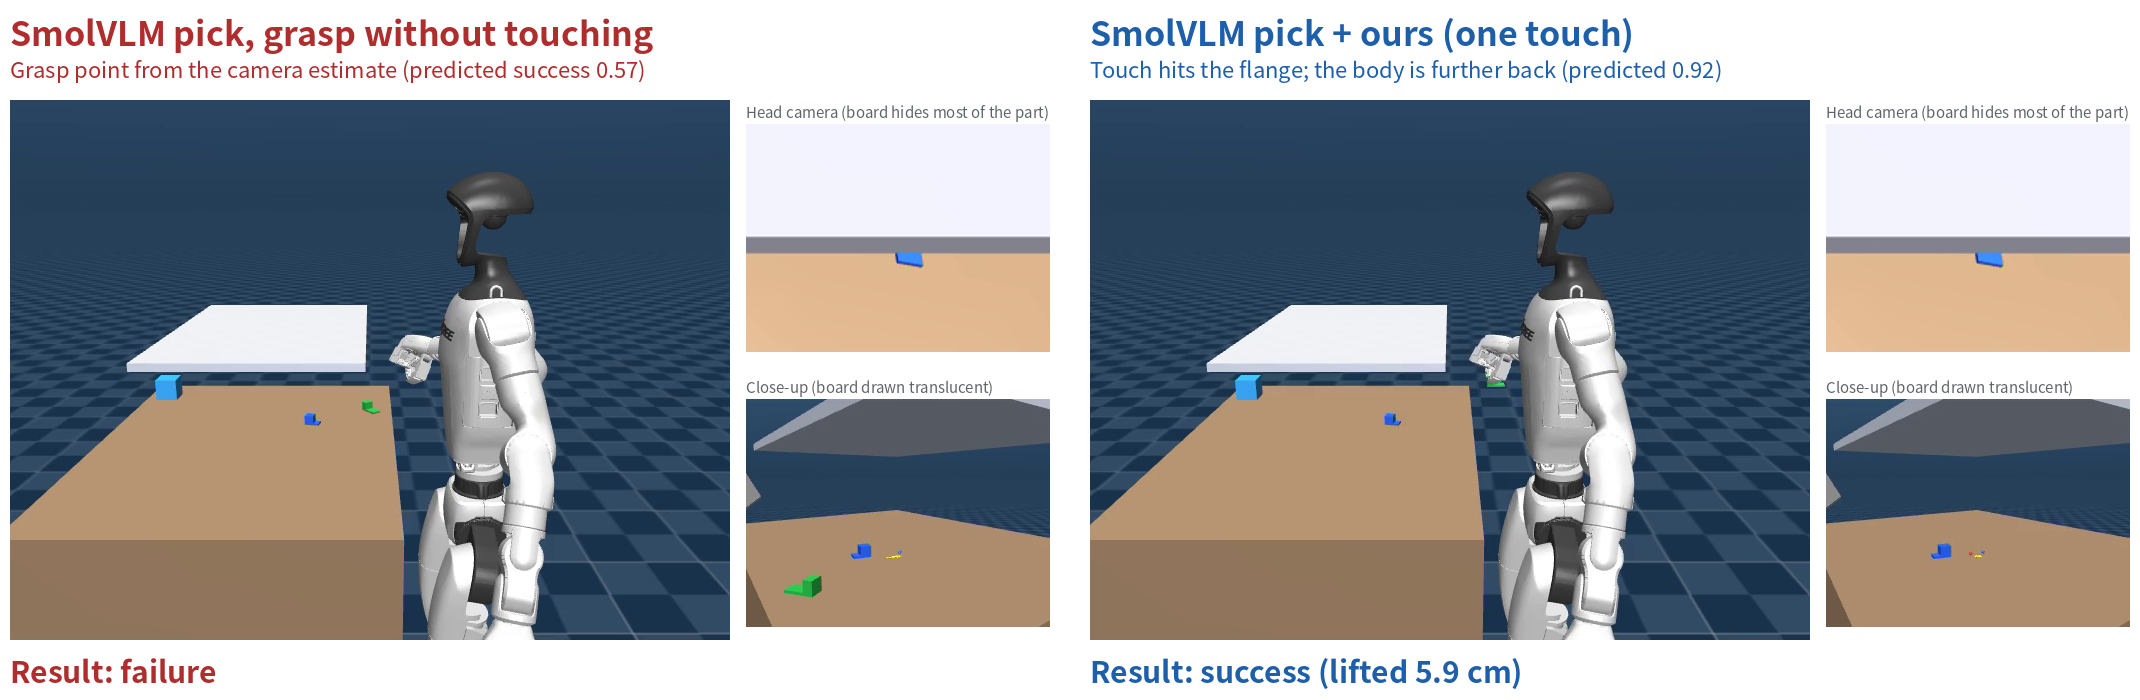
\includegraphics[width=0.95\textwidth]{figures/vlm_compare.png}
\caption{Same scene, same SmolVLM answer (``2'', the green part: flange 28\,mm, body 13\,mm). Left: grasping from the camera estimate without touching fails. Right: one touch lands on the flange, revealing that the body lies further back, and the grasp succeeds. The arm motion is identical; only the touch differs.}
\label{fig:vlm}
\end{figure*}

We then compared how to grasp the chosen part on 60 layouts $\times$ 2 parts = 120 trials (hidden sizes drawn from the predictor's training ranges; other settings as in Sec.~\ref{sec:setup}). All conditions are evaluated from the same observation by branching, and the part choice is assumed correct. For the VLM-grasp conditions, six candidate points A--F (8--48\,mm behind the estimated front face, every 8\,mm) are drawn on the image and SmolVLM chooses one zero-shot.

\begin{table}[h]
\caption{Choosing the grasp point for the picked part (120 trials)}
\label{tab:vlm}
\centering
\small
\begin{tabular}{@{}lc@{}}
\toprule
Grasp point chosen by & Success \\
\midrule
SmolVLM-500M, no part knowledge & 0.8\% \\
SmolVLM-2.2B, no part knowledge & 0.8\% \\
SmolVLM-500M, length ranges given in text & 43.3\% \\
SmolVLM-2.2B, length ranges given in text & 61.7\% \\
Learned predictor, no touch & 75.8\% \\
Ours, one touch & 95.0\% \\
\bottomrule
\end{tabular}
\end{table}

Without part knowledge, SmolVLM-500M answered only A or F and SmolVLM-2.2B only F, and almost nothing was lifted. Given the flange and body length ranges, the candidate distances, and the required margin in text, the models chose middle points, but SmolVLM-2.2B answered only C or D, comparable to always choosing C (57\%) or D (65\%). The body is hidden by the board, so the image offers no cue for moving the grasp point per layout. The learned predictor, which uses the same camera estimate, reached 75.8\%, 14.2 points above SmolVLM-2.2B (discordant 32 vs.\ 15, McNemar $p=0.019$). One touch raised success to 95.0\%, 19.2 points above the predictor without touching (95\% CI [+11.7, +26.7]; discordant 25 vs.\ 2; $p<0.001$); at $v=10$\,mm it rose from 63\% to 93\%. Both prompts are given verbatim in \texttt{run\_vlm\_point.py}.

\section{Reproduction}\label{app:repro}
Code, the trained predictor, all raw results, and videos are at \url{https://github.com/Nishina-N/Physics-Informed-Touch-Selection}. The environment is Python 3.11 with MuJoCo 3.14, mink 1.3, and scikit-learn 1.8.0 (locked in \texttt{uv.lock}).
\begin{footnotesize}
\begin{verbatim}
uv sync
git clone https://github.com/google-deepmind/\
mujoco_menagerie third_party/mujoco_menagerie
git -C third_party/mujoco_menagerie checkout \
  c96a32d28fb5da84da38c1da4d749e7a13212855
# numbers from the stored results (seconds)
uv run python analyze_touchsel.py
uv run python analyze_branch.py
# retrain the predictor (seconds)
uv run python train_predictor.py
# rerun everything (k = 0..n-1 in parallel)
uv run python gen_grasp_data.py 0 2 8000
uv run python run_touchsel.py 0 2 240 predictor.pkl
TSEL_RULES=geom uv run python run_touchsel.py \
  0 2 240 predictor.pkl
uv run python run_branch.py 0 2 120 predictor.pkl
\end{verbatim}
\end{footnotesize}
Expected outputs: \texttt{analyze\_touchsel.py} prints success 0.954 (\Ours), 0.887 (\Unc; 213/240 = 88.75\%, reported as 88.8\%), and a paired difference of +0.067 with McNemar $p=0.005$; \texttt{analyze\_branch.py} prints 0.725 for A, 0.967 for B1, and the C(0.85)$-$B1 difference; \texttt{paper/make\_numbers.py} and \texttt{paper/make\_figures.py} regenerate the ablation numbers and result figures; \texttt{train\_predictor.py} prints Brier 0.044 and accuracy 0.943 and reproduces \texttt{predictor.pkl}. Layouts are fixed by seeds, so a rerun of layout 0 reproduces the stored result exactly. On one CPU core, generating the training data takes about 3.5\,h, and the 120-layout touch-count experiment about 20\,min. \texttt{view\_trial.py 64 --rule voi} shows the trial of Fig.~\ref{fig:layout64}, and \texttt{docs/code\_guide.html} walks through the code in execution order.
